\documentclass[11pt, letterpaper, titlepage]{article}
\usepackage[utf8]{inputenc}
\usepackage[export]{adjustbox}
\usepackage{geometry}
 \geometry{
 a4paper,
 total={168mm,257mm},
 left=20mm,
 top=15mm,
 includefoot,includehead
 }


\usepackage[backend=biber, style=authoryear, giveninits=true, maxbibnames=25, uniquename=init, maxcitenames=2, hyperref=true, dashed=false]{biblatex}			% Benutze Biber/BibLaTeX zum Zitieren
\addbibresource{main.bib}					% Pfad zur BibTeX Datei aus Citavi
\renewcommand{\cite}{\parencite}
\usepackage{caption}
\usepackage{subcaption}
\usepackage{graphicx}
\usepackage{svg}
\usepackage{placeins}
\usepackage[hidelinks]{hyperref}
\usepackage{amsmath}
\usepackage[headsepline]{scrlayer-scrpage}
\usepackage{acronym}

\clearpairofpagestyles %Seitenzahl nicht in der Kopfzeile
\title{MeetEU Project - Team Heidelberg - Team 1 -- \\ Identification and Enhancement of novel Sars-CoV-2 NSP13 Helicase Inhibitors}
\author{Linda Blaier, Paul Brunner, Selina Ernst, Valerie Segatz, and Chlo\'{e} Weiler}
\date{February 2024}

%%%%%%%%%%%%%%%%%%%%%%% SELINA
\usepackage{tabularray}
\DeclareUnicodeCharacter{2009}{\,}

\begin{document}

\maketitle

\ihead{\headmark}
\automark{section}  %Kopfzeile gleich dem Sektiontitel
\cfoot{\pagemark}   %\ofood Seitenzahl rechts

\section{Abstract}
Even though the development of vaccines against Sars-CoV-2 was successful during the recent pandemic, the amount of FDA approved drugs for the therapy of Covid-19 is still limited to Paxlovid and Veklury, Olumiant and Actemra \cite{FDACOVID}. One possibility to accelerate the development of new therapies for Covid19 is to screen already approved drugs for effects against the viral reproduction. In this years MeetEU project, we investigated the NSP13 helicase of Sars-CoV-2 and tried to find compounds that could be repurposed for this therapy, as well as novel compounds that could lead to an effective treatment of Covid19. Using our \textit{in-silico} pipeline enables us to evaluate possible drug candidates, suggest novel structures based on already approved drugs and investigate their toxicity, while being cheaper and less labor intensive than projects limited to wet-lab work. 
\FloatBarrier

\newpage
%    Abkürzungsverzeichnis
{\setlength{\parskip}{0.2cm}
\section*{Abbreviations}
    \begin{acronym}[LC-MS/MS23]
        % A B C D E F G H I J K L M N O P Q R S T U V W X Y Z        
        % Abkürzungen
    \acro{COVID-19}{coronavirus disease 2019}
    \acro{FDA}{food and drug administration}
    \acro{MD}{molecular dynamics}
    \acro{MM-PBSA}{molecular mechanics energies combined with the Poisson-Boltzmann and surface area continuum solvation}
    \acro{NSP13}{non-structural protein 13}
    \acro{RMSD}{root mean square deviation}
    \acro{RMSF}{root mean square fluctuation}
    \acro{RTC}{replication transcription complex}
    \acro{SARS-CoV-2}{severe acute respiratory syndrome coronavirus type 2}
    \acro{SAscore}{synthetic accessibility score}
    \acro{ssRNA}{single-stranded RNA}
    \acro{Vina}{AutoDock Vina 1.1.2}
    \acro{ZBD}{zinc-binding domain}
       
        % Formelzeichen
        
        
        % als benutzt markierte Acronyme    
        
        
    \end{acronym}
}
\newpage
 
\section{Introduction}

\section{Material and Methods}

\subsection{Moecular Docking}
The molecular docking was done twice. 
% First as an initial screening of all 5092 prepared ligands (1472 from the ZINC database, 3620 from the ECBD database).
% ECBD pdbqt: 3813 (problematic: 193) = 3620 (size: 28) = 3592
% ZINC pdbqt: 1567 (problematic: 95) = 1472 (size: 44) = 1428
For the initial screening of the ligands \ac{Vina} was utilized \cite{Trott.2010}. As the receptor the monomer of 6ZSL was used which includes only chain A. Especially for \ac{Vina} the zinc ions were also removed and the resulting structure was converted into the pdbqt format through AutoDockTools 1.5.7 \cite{Goodsell2021}. The consensus pocket was introduced as the grid box with lengths of 30 \AA. The exhaustiveness was set to 30 and the maximum number of binding modes to 9. Taking advantage of multithreading, \ac{Vina} uses the 28 CPUs accessible on the multi-core server \cite{Che2023}. A filter was applied on the set of ligands assuring only 3D structures smaller than the specified grid box were screened against the receptor (1428 from the ZINC database and 3592 from the ECBD database). The filter was implemented in Python 3.11.6 and executed together with the \ac{Vina} command in Bash script. The resulting 9 different conformations for each ligand were ranked by their affinity scores and only the best value was considered in further steps. A number of ligands were later found to have multiple docking results due to an overlap between the two datasets and in accordance with previous steps only the best score was kept. The remaining 4862 ligands were ranked by their affinity score and the top one hundred were selected for next steps. \\
A second molecular docking was performed with those top scorers from the screening as well as ADP and ATP. The docking software Glide provided by Schrödinger Inc \cite{Friesner2004}. was accessed through Maestro 2022.3 \cite{Maestro2022}. The included tools Protein Preparation Wizard and LigPrep \cite{Madhavi2013} were utilized to prepare the monomer helicase and ligands for the docking process with the OPLS4 force field \cite{Lu2021}. The pH value was set to 7.0. The ligand preparation generates depending on the initial structure a varying amount of conformations. In the analysis of the results only the best performing conformation was included. The Receptor Grid Generation panel was used to generate the receptor grid with the same binding pocket as in \ac{Vina}. The docking with Glide was performed at standard precision (SP) mode and with flexibility of the ligands enabled \cite{Halgren.2004}. The criteria for the selection of the best performing ligands was chosen to be the docking score. The interactions between the top scoring ligands and the receptor were noted down. 


\section{Results}

\subsection{Screening of ligands with AutoDock Vina}
A library of 5020 ligands was screened against the consensus binding pocket of the NSP13 helicase. The best conformation with the lowest binding affinity was determined for each one of these ligands. 157 of them were included two or three times. The respective difference of affinity between the multiple forms of each ligand never exceeded 1.6. In 24.2 \% of these cases the affinity score remained the same. Whenever the difference is not equal to zero the corresponding rank of the affinities changed with a maximum margin of 2966. In the case of multiple runs for each ligand the best scoring docking result was kept. The remaining 4862 had affinity values ranging from -10.3 to -2.4. The ranking of the ligands was determined by their affinity which lead to the selection of the top one hundred ligands. Their values ranged from -10.3 to -8.8. Containing 2.1 \% of all ligands these top scorers are only the preselection for the subsequent docking process. 

\subsection{Molecular Docking of top scorers with Glide}
The 100 top scorers from the screening were subjected to another molecular docking to the NSP13 helicase. The resulting docking scores from Glide were utilised to establish another ranking. The comparison of the results from Vina and Glide showed that there was no correlation between these ranks (\autoref{fig:comp_glide_vina}). The Pearson correlation coefficient r of the scores is 0.13 with a p-value of 0.19 which is similar to the r value of the ranks at 0.12 with a p-value of 0.22. The Kendall correlation coefficient computed by comparing the ranks only is 0.07 with a p-value of 0.25. In all three cases it is not possible to reject the null hypothesis of no correlation. Even so, there are 3 from the top 5 Vina scorers (rank 1, 2 and 4) that are also part of the top 10 (rank 9, 10 and 8) according to Glide. Moving forward docking scores from Glide are the preferred selection criteria since Glide provided flexibility of ligands and the retainment of the protein zinc ions. \\

% for appendix
\begin{figure}[htp]
	\centering
	\captionsetup[subfigure]{skip=-20pt,position=top,labelfont=bf,labelformat=parens,singlelinecheck=false}
	\subcaptionbox{%
		\label{subfig:comp_ranks}}{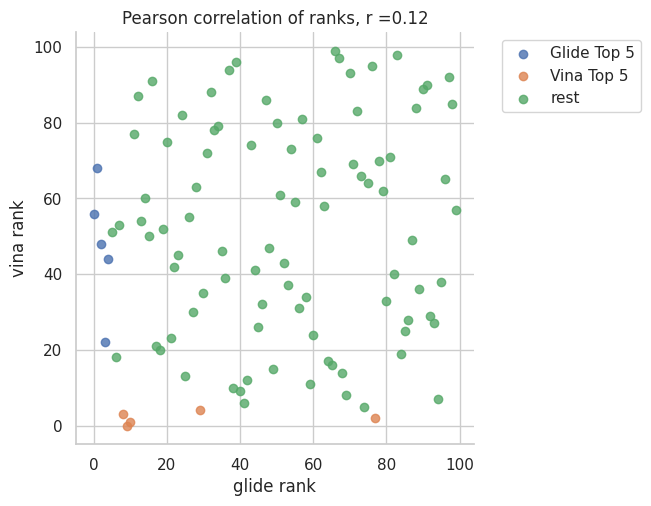
\includegraphics[scale=0.5]{img/Comparison_of_ranks.png}}
	\subcaptionbox{%
		\label{subfig:comp_scores}}{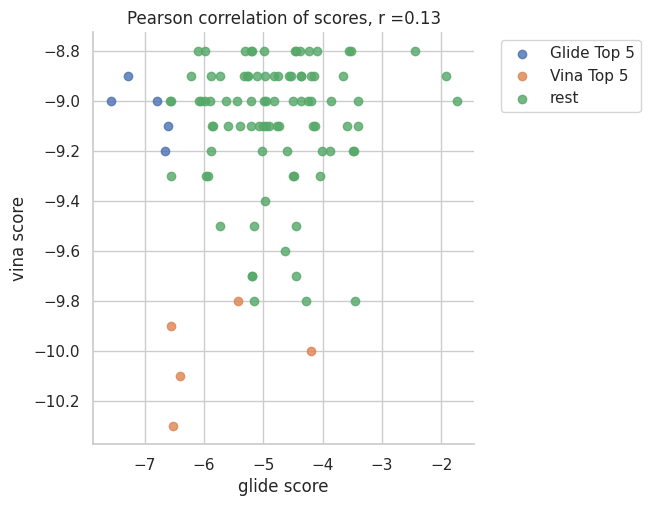
\includegraphics[scale=0.5]{img/Comparison_of_scores.png}}
	\caption{Comparison of Vina and Glide docking results. 100 ligands were compared in  \subref{subfig:comp_ranks}) ranks and \subref{subfig:comp_scores}) docking scores. Dots in blue represent the top 5 ligands from Vina and in orange the top 5 from Glide. All the other ligands are marked green.}\label{fig:comp_glide_vina}
\end{figure}

The potential lead compounds defined in this way are as follows: Angiotensin 1-7 (ECBD ID: EOS100380, ZINC ID: ZINC000096077632), ZINC000008101127 (ECBD ID: not existent) and VX-11 (ECBD ID: EOS100897, ZINC-ID: ZINC000035880991). Each one of these ligands has a better docking score and therefore higher affinity to the receptor than ADP (\autoref{tab:top_docking_scores}). However ATP still binds better than any one them.

% for appendix
\begin{table}[htp]
	\centering
	\caption{Glide docking scores for the top 4 ligands, ATP and ADP.}\label{tab:top_docking_scores}
	\begin{tblr}{
			hline{1-2,12} = {-}{},
		}
		 Title            & docking score \\
		 ATP              & -7.991        \\
		 EOS100380        & -7.573        \\
		 ZINC000008101127 & -7.273        \\
		 EOS100897        & -6.786        \\
		 ZINC000150588351 & -6.655        \\
		 ADP              & -6.63         \\   
	\end{tblr}
\end{table}

Another output are the iintermolecular interactions between the small molecules and the receptor binding pocket. Interesting to note is that especially ATP, ADP and the highest top scorer EOS100380 have many common 
bonds with the amino acids like LYS 288, LYS 320 and ARG 443 (\autoref{tab:ligand_interactions}). In most cases these bonds are either hydrogen bonds or salt bridges with some exceptions like an aromatic hydrogen bonds, halogen bonds or pi-cation. One amino acid in particular stands out which is LYS 288 that also interacts with the other top 3 scorers ZINC000008101127 and EOS100897. 

\begin{table}[htp]
	\centering
	\caption{List of intermolecular interactions between ligands and receptor protein.}\label{tab:ligand_interactions}
	\begin{tblr}{
			hline{1-2,16} = {1-3}{},
		}
		Ligand           & Bond type       & Amino acid                                                        &  \\
		ADP              & hydrogen bond   & {GLY 287, LYS 288, SER 289, HIE 290, \\LYS 320, ARG 443, SER 539} &  \\
		& aromatic h-bond & LYS 320                                                           &  \\
		& salt bridge    & LYS 288, LYS 320, ARG 443                                         &  \\
		& Pi-cation       & ARG 443                                                           &  \\
		ATP              & hydrogen bond   & {GLY 287, LYS 288, SER 289, HIE 290, \\ARG 443, GLH 375}          &  \\
		& salt bridge    & LYS 288, LYS 320, ARG 443                                         &  \\
		EOS100380        & hydrogen bond   & {LYS 288, LYS 320, ASP 315, GLU 319, \\GLU 341, ARG 443, GLU 540} &  \\
		& salt bridge    & {LYS 288, LYS 320, ASP 315, GLU 319,~ \\ARG 443, GLU 540}         &  \\
		ZINC000008101127 & hydrogen bond   & ARG 178                                                           &  \\
		& aromatic h-bond & GLY 538                                                           &  \\
		& salt bridge    & LYS 288                                                           &  \\
		EOS100897        & hydrogen bond   & ASP 534                                                           &  \\
		& halogen bond    & ASN 516, THR 532                                                  &  \\
		& Pi-cation       & LYS 288                                                           &  
	\end{tblr}
\end{table}

When comparing the overall positions of EOS100380 (\autoref{fig:docking_EOS100380}) and ADP (\autoref{fig:docking_ADP}) within the binding pocket the similarities are even more apparent. 

% for appendix
\begin{figure}[htp]
	\centering
	\captionsetup[subfigure]{skip=-20pt,position=top,labelfont=bf,labelformat=parens,singlelinecheck=false}
	\subcaptionbox{%
		\label{subfig:EOS100380}}{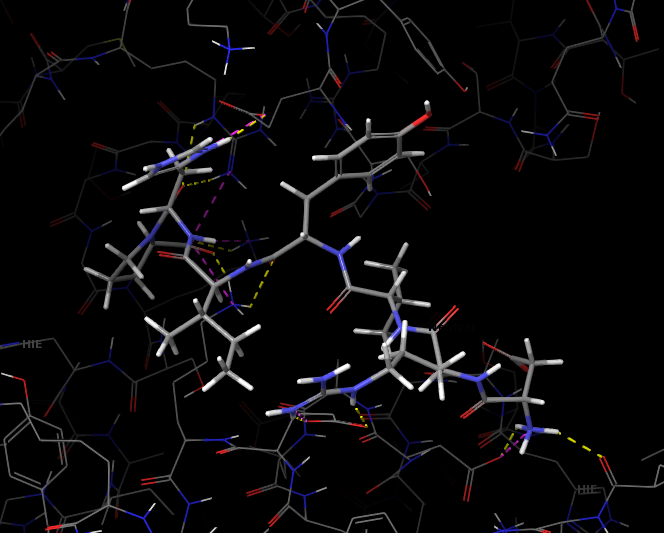
\includegraphics[scale=0.5]{img/docking_EOS100380.png}}
	\subcaptionbox{%
		\label{subfig:EOS100380_s}}{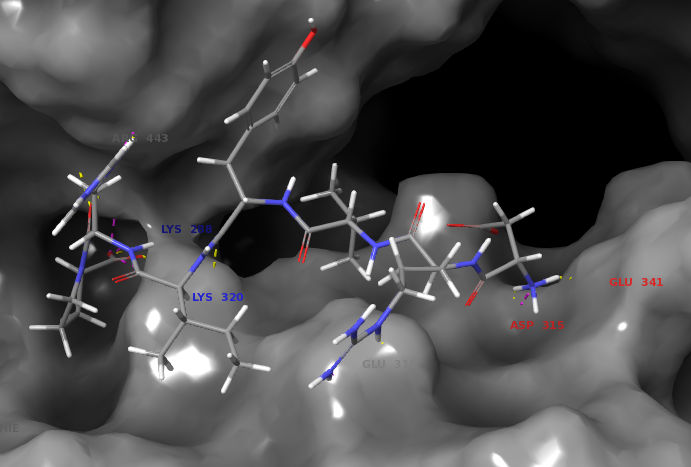
\includegraphics[scale=0.57]{img/docking_EOS100380_surface.png}}
	\caption{Molecular docking of the top scoring ligand with Glide. The result of the docking process with the top scoring ligand (ECBD ID: EOS100380) is shown with focus on \subref{subfig:EOS100380}) the specific interactions between ligand and receptor protein and \subref{subfig:EOS100380_s}) position within the binding pocket. The different interactions between the two molecules are coloured depending on type. Hydrogen bonds are shown as yellow and salt bridges as violet.}\label{fig:docking_EOS100380}
\end{figure}

% for appendix
\begin{figure}[htp]
	\centering
	\captionsetup[subfigure]{skip=-20pt,position=top,labelfont=bf,labelformat=parens,singlelinecheck=false}
	\subcaptionbox{%
		\label{subfig:ADP}}{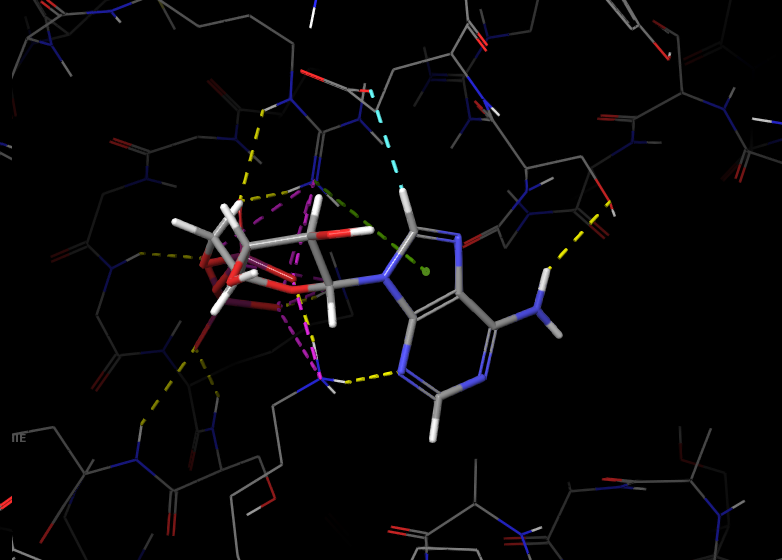
\includegraphics[scale=0.45]{img/docking_adp.png}}
	\subcaptionbox{%
		\label{subfig:ADP_s}}{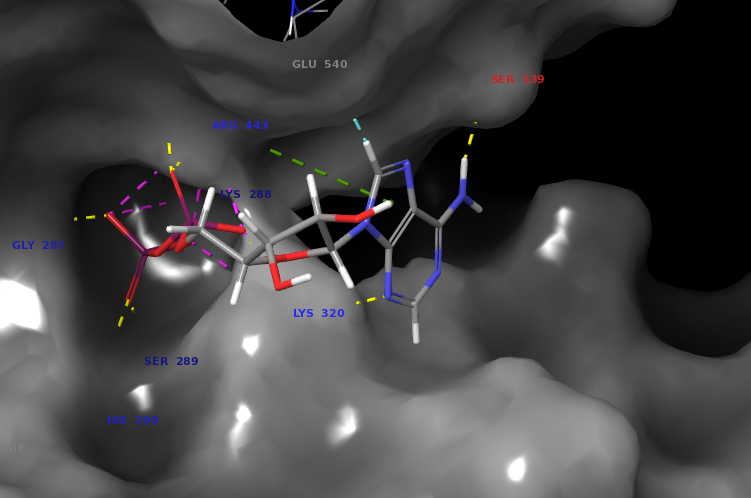
\includegraphics[scale=0.5]{img/docking_ADP_surface.png}}
	\caption{Molecular docking of the ADP with Glide. The result of the docking process with ADP is shown with focus on \subref{subfig:ADP}) the specific interactions between ligand and receptor protein and \subref{subfig:ADP_s}) position within the binding pocket. The different interactions between the two molecules are coloured depending on type. Hydrogen bonds are shown as yellow, salt bridges as violet, aromatic hydrogen bonds as blue and pi-cation as green.}\label{fig:docking_ADP}
\end{figure}


\subsection{Comparison of AutoDock Vina results}
%This part only makes sense if they actually used the same pocket? Don't think they used the same 6zsl structure ...
The Team Sorbonne5 also used AutoDock Vina for the docking of ligands from the pilot library of the ECBD database. Most of these ligands were also included in the former mentioned analysis. With the exception of two it is possible to map the top 10 ligands from Sorbonne to results of the analysis. Only one of their top scorers is included in the 100 preselected ligands. Their first ranked ligand with the affinity score -11.1 has a corresponding rank of 63. The remaining 7 were mapped to lower ranks starting with 123 and ending with up to 2626.

\FloatBarrier

\section{Discussion and Outlook}

\section{Supplementary Material}

\pagebreak
\FloatBarrier
\renewcommand{\bibname}{References}  % damit Literatuverzeicnis mit "References" betitelt
\printbibliography
\end{document}
